\documentclass[onecolumn]{aastex62}


\newcommand{\vdag}{(v)^\dagger}
\newcommand\aastex{AAS\TeX}
\newcommand\latex{La\TeX}
\usepackage{listings}
\usepackage{amsmath}
\usepackage{physics}
\usepackage{hyperref}
\usepackage{natbib}
\usepackage[T1]{fontenc}
\usepackage[english]{babel}
\usepackage[utf8]{inputenc}

\begin{document}

\title{\Large Milestone III:\\Integrating the initial perturbations.}


\author{Håkon Tansem}

\section{Introduction} \label{sec:intro}
This is the third milestone in a four milestone project where the end goal is to compute the CMB power spectrum. In the previous two milestones we have solved for the background evolution of the universe(). In this third milestone we will study how perturbations has evolved throughout cosmic history. We will start with the initial conditions as predicted by inflation and solve the equations for baryons, cold dark matter and photons as well as the metric perturbations given by the Boltzmann equations and Einsteins equations.
\section{Method} \label{sec:method}
In this model we assume a few simplifications. We neglect photon polarization and ignore neutrinos as to reduce the number of equations. We will therefore only study the evolution of the density parameter $\delta$ and velocity parameter $v$ for baryons and dark matter, the perturbation to the photon distribution $\theta_{\ell}$, where we include integer multipoles $\ell\in[0, 7]$, as well as the metric perturbations $\Phi$ and $\Psi$ all as functions of $x=log(a)$. When studying the perturbations we will work in fourier space where each mode is denoted by the magnitude of its wavevector $k$. When integrating the perturbations we have two main regimes to take into account. In early times, as we calculated in milestone II, we saw that the optical depth of the universe $\tau\gg1$ due to all electrons being free. This means that at any given point in space the mean free path for a photon is very small. This gives very little anisotropy as only perturbations very close by can be observed. This suppresses all higher multipoles and washes out their gradients making only $\ell=0$ and $\ell=1$ the nonnegligible moments. This makes photons behave like a fluid described by the two variables density and velocity which in our case is represented by $\theta_0$ and $\theta_1$ respectively \citep[p. 225]{Dodelson:1282338}. As criterions for deciding wether we are in the tight coupling regime we check wether we are past the onset of recombination, at which time we approximate by evualuating the free electron fraction $X_e$ and seeing wether it is smaller than $0.99$, or if the criterion $\left|\frac{d\tau}{dx}\right| < 10 \cdot \text{min}(1, \frac{ck}{\mathcal{H}})$ is met. That is if $X_e < 0.99$ or if the criterion is met, we assume that we are no longer in the tight coupling regime.\\\indent

When solving the equations we start by setting the initial conditions given by inflation as
\begin{align}
    \Psi &= -\frac{2}{3}\\
    \Phi &= -\Psi \\
    \delta_{\rm CDM} &= \delta_b = -\frac{3}{2} \Psi \\
    v_{\rm CDM} &= v_b = -\frac{ck}{2\mathcal{H}} \Psi\\
    \Theta_0 &= -\frac{1}{2} \Psi \\
    \Theta_1 &= +\frac{ck}{6\mathcal{H}}\Psi \\
    \Theta_2 &= -\frac{20ck}{45\mathcal{H}\tau^\prime} \Theta_1,\label{eq:t2init}\\
    \Theta_\ell &= -\frac{\ell}{2\ell+1} \frac{ck}{\mathcal{H}\tau^\prime} \Theta_{\ell-1}.\label{eq:tellinit}\\
\end{align}
All equations in this paper are given by \cite{WintherIII:2020} unless otherwise stated. The full set of ODE's for the photon multipoles are given as
\begin{align}
    \Theta^\prime_0 &= -\frac{ck}{\mathcal{H}} \Theta_1 - \Phi^\prime,\label{eq:tp1} \\
    \Theta^\prime_1 &=  \frac{ck}{3\mathcal{H}} \Theta_0 - \frac{2ck}{3\mathcal{H}}\Theta_2 +
    \frac{ck}{3\mathcal{H}}\Psi + \tau^\prime\left[\Theta_1 + \frac{1}{3}v_b\right], \\
    \Theta^\prime_\ell &= \frac{\ell ck}{(2\ell+1)\mathcal{H}}\Theta_{\ell-1} - \frac{(\ell+1)ck}{(2\ell+1)\mathcal{H}}
    \Theta_{\ell+1} + \tau^\prime\left[\Theta_\ell - \frac{1}{10}\theta_2
    \delta_{\ell,2}\right], \quad\quad 2 \le \ell < \ell_{\textrm{max}} \\
    \Theta_{\ell}^\prime &= \frac{ck}{\mathcal{H}}
    \Theta_{\ell-1}-c\frac{\ell+1}{\mathcal{H}\eta(x)}\Theta_\ell+\tau^\prime\Theta_\ell,
    \quad\quad \ell = \ell_{\textrm{max}}.\\
\end{align}
where $\delta_{\ell,2}$ is the kroenecker-delta and $\eta(x)$ is the conformal time computed in milestone I. For cold dark matter and baryons as well as the metric perturbations, we have
\begin{align}
    \delta_{\rm CDM}^\prime &= \frac{ck}{\mathcal{H}} v_{\rm CDM} - 3\Phi^\prime \\
    v_{\rm CDM}^\prime &= -v_{\rm CDM} -\frac{ck}{\mathcal{H}} \Psi \\
    \delta_b^\prime &= \frac{ck}{\mathcal{H}}v_b -3\Phi^\prime \\
    v_b^\prime &= -v_b - \frac{ck}{\mathcal{H}}\Psi + \tau^\prime R(3\Theta_1 + v_b) \\
    \Phi^\prime &= \Psi - \frac{c^2k^2}{3\mathcal{H}^2} \Phi + \frac{H_0^2}{2\mathcal{H}^2}
    \left[\Omega_{\rm CDM} e^{-x} \delta_{\rm CDM} + \Omega_{b,0} e^{-x} \delta_b + 4\Omega_{r,0}
    a^{-2}\Theta_0\right] \\
    \Psi &= -\Phi - \frac{12H_0^2}{c^2k^2e^{2x}}\Omega_{r,0}\Theta_2, \\
\end{align}
where $R = \frac{4\Omega_{r,O}}{3\Omega_{b,0}e^x}$. These equations apply as they are written when we have exited the tight coupling regime. In the tight coupling regime, as described earlier, multipoles larger than $\ell=1$ have their gradients washed out. This gives the following changes to the set of equations 
\begin{align}
    q &= \frac{-[(1-R)\tau^\prime + (1+R)\tau^{\prime\prime}](3\Theta_1+v_b) -
    \frac{ck}{\mathcal{H}}\Psi + (1-\frac{\mathcal{H}^\prime}{\mathcal{H}})\frac{ck}{\mathcal{H}}(-\Theta_0 +
    2\Theta_2) - \frac{ck}{\mathcal{H}}\Theta_0^\prime}{(1+R)\tau^\prime + \frac{\mathcal{H}^\prime}{\mathcal{H}} -
    1}\\
    v_b^\prime &= \frac{1}{1+R} \left[-v_b - \frac{ck}{\mathcal{H}}\Psi + R(q +
    \frac{ck}{\mathcal{H}}(-\Theta_0 + 2\Theta_2) - \frac{ck}{\mathcal{H}}\Psi)\right]\\
    \Theta^\prime_1 &= \frac{1}{3} (q - v_b^\prime).
\end{align}
Note that $\Theta^\prime_0$ is still the same as given by equation \ref{eq:tp1}.  In the tight coupling regime the higher order multipoles are given by their initial as shown in equations \ref{eq:t2init} and \ref{eq:tellinit}. The differential equations given are solved numerically for every fourier mode $k$ given in a logarithmically spaced intervall between $k_min=$ and $k_max=$. Each fourier mode is solved on a linearly spaced $x-$interval ranging from $x_min=log(1e-8)$ to present time at $x_max=0$. The solution for each fourier mode for all of the components are stored so that they can ble splined. This gives us the ability to evaluate each component for an arbitrary $x$ and $k$ value.
\section{Results}
\label{sec:results}
All results were produced using a cosmology with $\Omega_{b,0}=0.05$, $\Omega_{cdm,0}=0.25$ and $\Omega_{\Lambda,0}=0.7$ and $h=0.7$. From using data from milestone I matter-radiation equality $a_{eq}$ was calculated to correspond to $x=-8.68$ which will be used in most results as a reference point. To illustrate three different regimes relative to horizon entry three fourier modes $k=0.001$, $k=0.05$ and $k=0.3$ were chosen to present the main results.

When solving the equations for the metric perturbations $\Phi$ and $\Psi$ for the different fouries modes $k$, our model produced the results shown in figure \ref{fig:Psi}. Further we have the solutions for the density and velocity parameters for baryons and cold dark matter for the three different fourier modes illustrated in figures \ref{fig:delta} and \ref{fig:v} respectively. The results for the monopole $\theta_0$ and multipole $\theta_1$ is presented in figure \ref{fig:t0} and figure \ref{fig:t1}. As a means to compare the monopole and $\delta_b$ parameter, they were both plotted in figure \ref{fig:comp0} for a fourier mode $k=0.1$. Here the first two maximas of the monopole is plotted as vertical lines to illustrate overlap with fluctuations in $\delta_b$.
\begin{figure}
    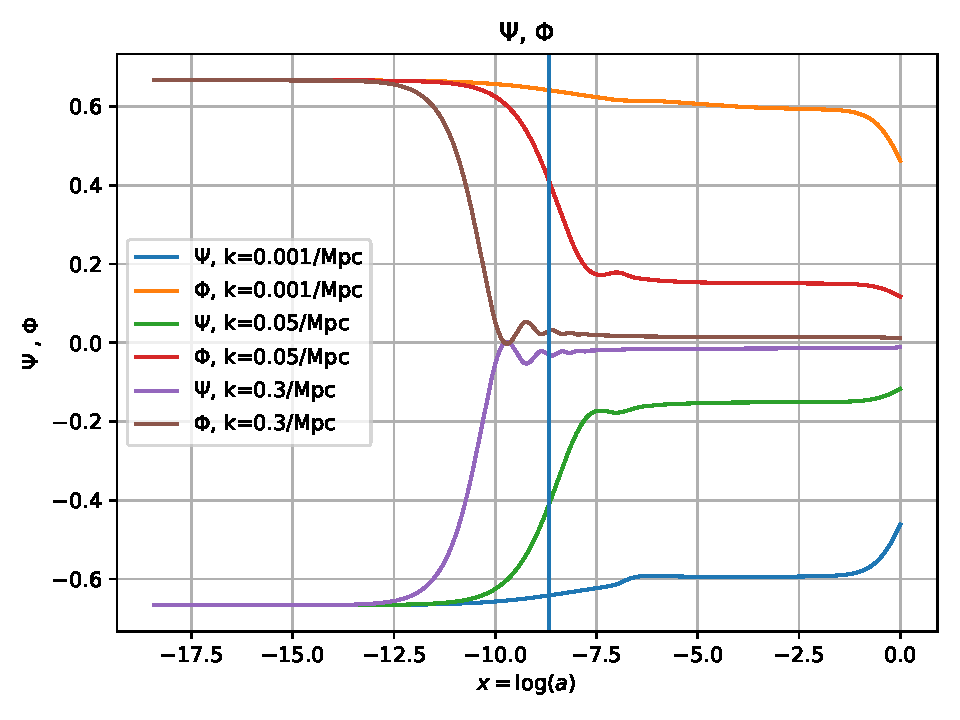
\includegraphics[scale=0.8]{figures/Psi.pdf}
    \caption{Figure showing the Metric perturbations $\Psi$ and $\Phi$ as functions of $x=log(a)$ for three different fourier modes $k$. The time $a_{eq}$ is plotted as a straight line}
    \label{fig:Psi}
\end{figure}

\begin{figure}
    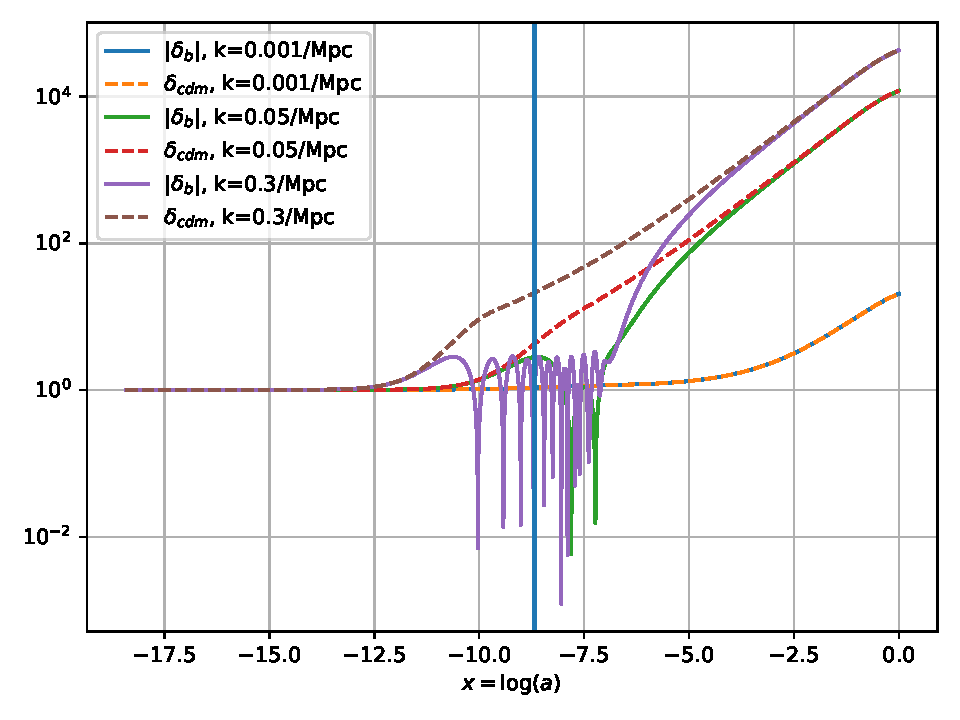
\includegraphics[scale=0.8]{figures/delta.pdf}
    \caption{Figure showing the $\delta$ parameter for baryons and cold dark matter as functions of x for three different fourier modes $k$. The time $a_{eq}$ is plotted as a straight line}
    \label{fig:delta}
\end{figure}

\begin{figure}
    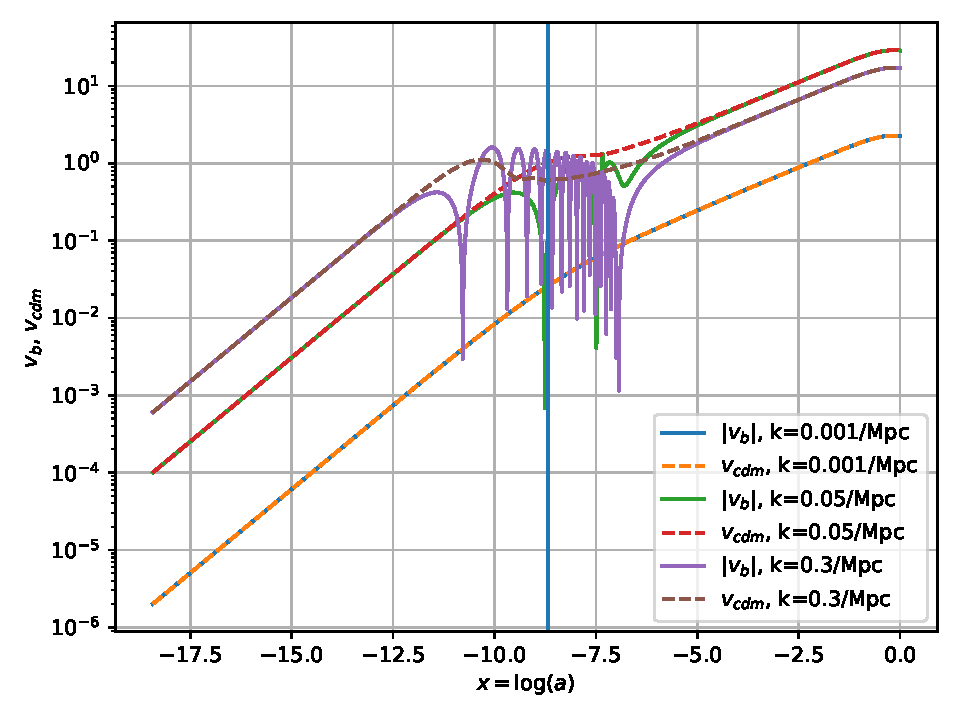
\includegraphics[scale=0.8]{figures/v.pdf}
    \caption{Figure showing the $v$ parameter for baryons and cold dark matter as functions of x for three fourier different modes $k$. The time $a_{eq}$ is plotted as a straight line}
    \label{fig:v}
\end{figure}

\begin{figure}
    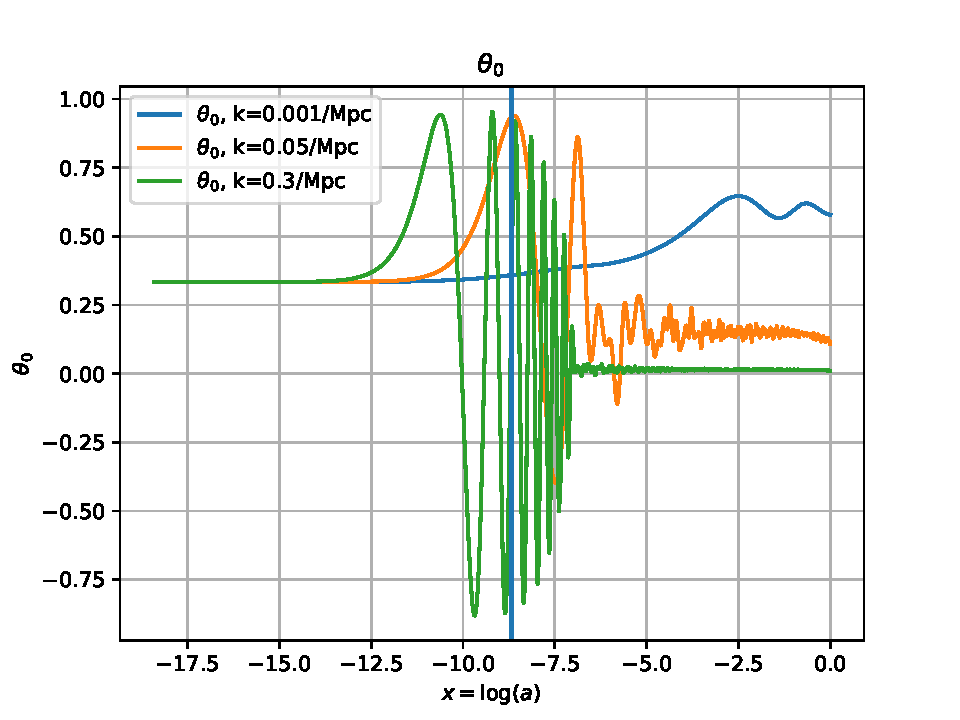
\includegraphics[scale=0.8]{figures/t0.pdf}
    \caption{Figure showing the monopole $\theta_0$ functions of x for three different fourier modes $k$. The time $a_{eq}$ is plotted as a straight line}
    \label{fig:t0}
\end{figure}

\begin{figure}
    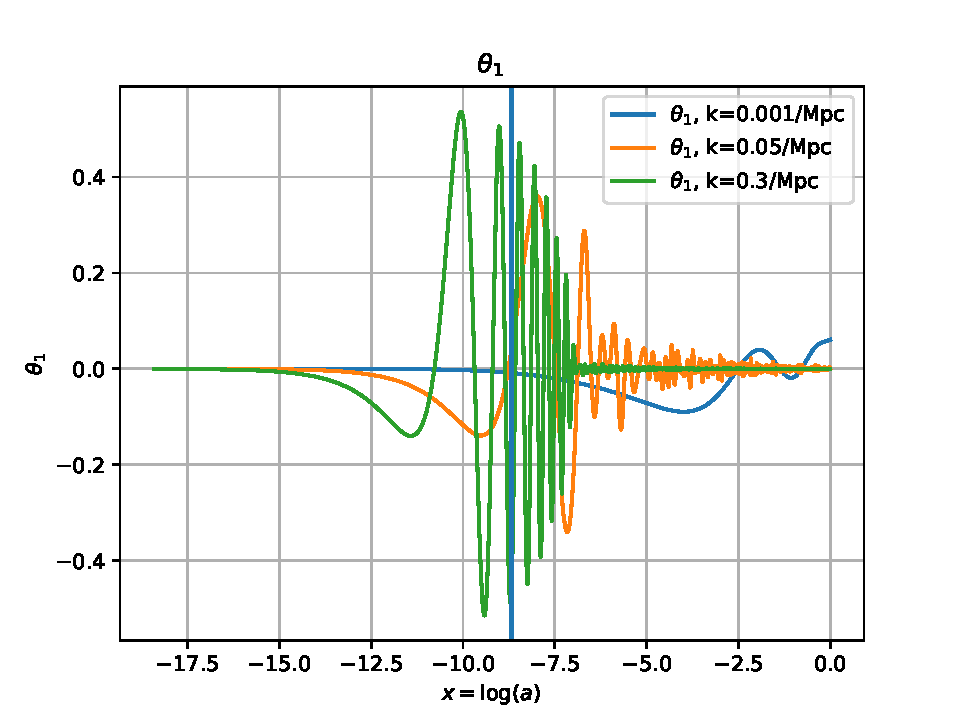
\includegraphics[scale=0.8]{figures/t1.pdf}
    \caption{Figure showing the multipole $\theta_1$ functions of x for three different fourier modes $k$. The time $a_{eq}$ is plotted as a straight line}
    \label{fig:t1}
\end{figure}

\begin{figure}
    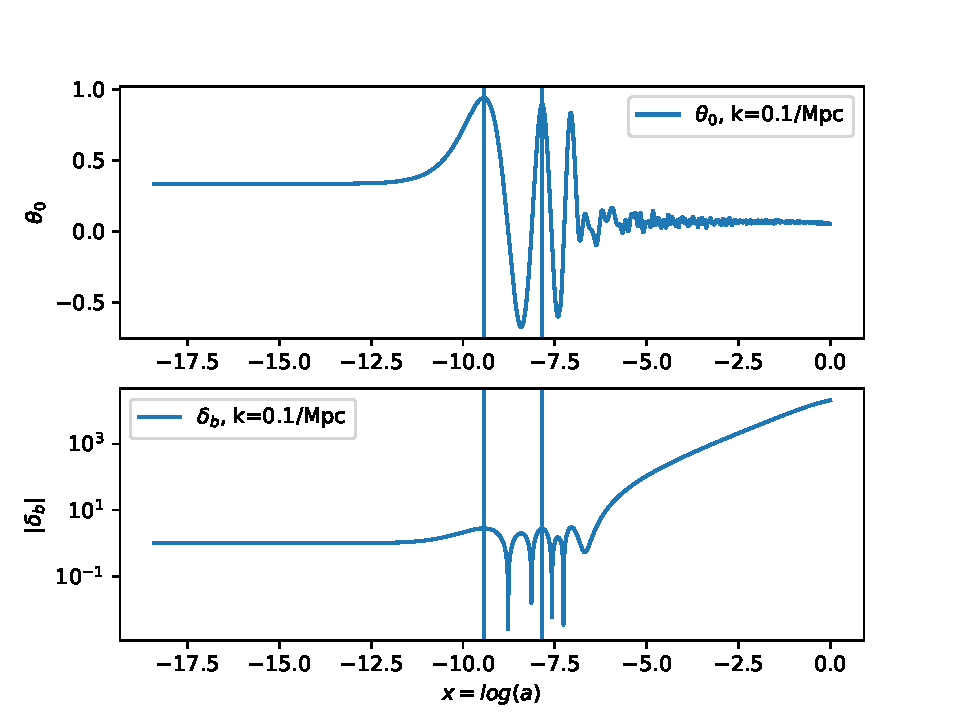
\includegraphics[scale=0.8]{figures/comparison0.pdf}
    \caption{Figure showing the monopole monopole $\theta_0$ as well as the density parameter for baryons $\delta_b$ for a fourier mode that completes a few oscillations before recombination. The first two maximas of the monopole is plottet as straight lines to illustrate overlap with maximas in the baryon density fluctuations.}
    \label{fig:comp0}
\end{figure}

\bibliography{ref.bib}
\bibliographystyle{aasjournal}
%\begin{thebibliography}{}
%\end{thebibliography}
\end{document}

% End of file `sample62.tex'.
